I 1982 begyndte man at arbejde på et ”anden generations”(2G) system indenfor mobiltelefoni og kaldte det for ”Groupe Spécial Mobile”(GSM). Inden da havde telekommunikation foregået analogt og sådan blev det ved indtil 1991, hvor denne digitale form for mobiltelefoni, GSM, blev sat i gang. Systemet blev hurtigt internationalt udbredt og man besluttede sig for at omdøbe det til ”Global System for Mobile communications”. Det er dog aldrig blevet til et globalt system idet man i Japan og USA bruger andre systemer \cite{denstoredanske}.

GSM netværket består af forskellige celler, som hver har en basestation, der kan modtage og sende signaler, se figur \ref{celler}. Basestations-controlleren, som ses på figur \ref{celler}, er ansvarlig for radio ressourcer for en eller flere basestationer. Basestations-controlleren har forbindelse til "mobile switching center", som er netværksenheder, som tager sig af den trådløse kommunikation. Basestationer dækker, med deres individuelle radius, hver især et geografisk område, altså en celle. Jo mindre radius en basestation har, jo større er dens tilgængelige båndbredde. Stationer som dækker byområder, kan derfor have en radius på helt ned til få hundrede metre mens stationer, som står længere ude på landet kan dække en radius på op til 30 kilometer. \cite{techviral}

\begin{figure}[H]
\centering
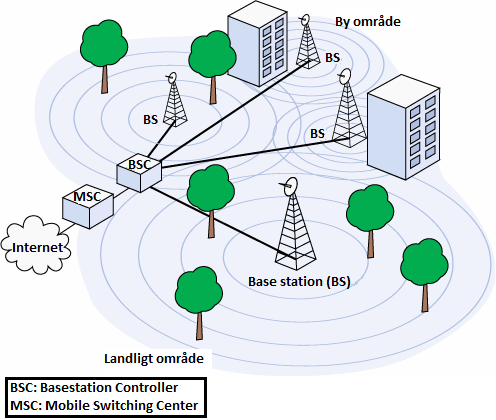
\includegraphics []{Billeder/celler.png}
\caption {Celler, som hver dækker deres eget geografiske område \cite{techviral}}
\label {celler}
\end{figure} 

Når man bruger sin mobiltelefon vil den, gennem luften, skabe kontakt til den nærmeste basestation, se figur \ref{GSM}. Hvis man har sendt en SMS-besked, vil denne modtages af basestationen, som sender den videre til SMS-centeret. SMS-centeret er herefter ansvarlig for at viderebringe SMS’en til modtageren. Hvis SMS-centeret ikke kan få forbindelse til modtagertelefonen (hvis denne er slukket eller udenfor signal), gemmes beskeden i centeret og sendes når der er oprettet forbindelse til modtageren. \cite{info}

\begin{figure}[H]
\centering
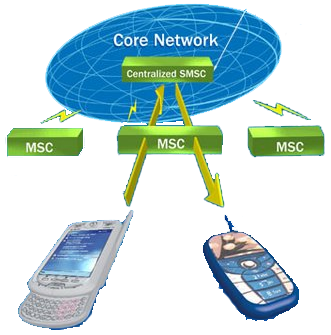
\includegraphics []{Billeder/GSMnetvaerk.png}
\caption {SMS'ens vej fra afsender til modtager \cite{info}}
\label {GSM}
\end{figure} 

I GSM er der indbygget to muligheder for at sende en flere af SMS-beskeder sammen. Den ene mulighed er SMS-sammenkædning, hvilket vil sige at en række SMS-beskeder bliver kædet sammen og sendes hver for sig, men hos modtageren bliver de sat sammen i korrekt rækkefølge og læses igen som én besked. Den anden mulighed er komprimering af tekst med Huffman coding \cite{UNI}. Hvis denne mulighed udnyttes kan man sende optil 80 tegn mere pr. SMS-besked. Dette kræver dog at telefonen fra fabrikkens side har sprogspecifike kompressionsparametre. Det har ikke været muligt at finde ud af om man idag reelt gør brug af denne mulighed for at komprimere tekstbeskeder. 
